\chapter{Deep learning primer}
\label{chap:Theory-Deep Learning}
This chapter provides a comprehensive explanation of foundational concepts and methodologies in deep learning, with a particular emphasis on Graph Neural Networks (GNNs). It begins by introducing deep learning and elucidating the basics of neural networks, focusing on their architecture and operational principles. Subsequently, it delves into optimization techniques, addressing essential elements such as loss functions, backpropagation, learning rates, and optimizers. Furthermore, it navigates through the intricacies of training neural networks with topics including data partitioning, feature scaling, weights initialization, regularization, batch training, and hyperparameter tuning. Additionally, this chapter examines model evaluation metrics and explores advanced neural network architectures such as Convolutional Neural Networks (CNNs) and Graph Neural Networks (GNNs), highlighting their important features and components. 

\section{Introduction to machine learning and deep learning}
Machine learning is a branch of artificial intelligence that focuses on developing algorithms capable of learning from data and improving their performance over time. The learning process utilizes statistical models and optimization algorithms to iteratively adjust parameters and improve performance. Machine learning approaches are broadly categorized into supervised learning and unsupervised learning based on learning objectives. \\

\textbf{Supervised learning} involves training a model using labeled data, where each input is paired with a corresponding output. During training, the model learns to map input data to output labels by minimizing the difference between its predictions and the true labels. This approach is commonly used for tasks such as classification and regression. \\

\textbf{Unsupervised learning}, in contrast, involves training a model on unlabeled data, where the algorithm aims to find hidden patterns or structures within the data without explicit guidance. Unsupervised learning is often used for tasks like anomaly detection, data exploration, and feature learning, where the data lacks labeled examples or where the underlying structure is unknown. \\

Deep learning is a subset of machine learning that has gained significant attention due to its remarkable performance in various tasks, ranging from image and speech recognition to autonomous driving. It utilizes neural networks consisting of multiple layers of interconnected neurons to learn representations of data through iterative processing of input data to make predictions or decisions. The key distinction between machine learning and deep learning lies in the depth and complexity of the models. We will exclusively delve into the specifics of supervised learning in this work. Henceforth, when we mention machine learning or deep learning, it refers to supervised learning in this context.
\section{Fundamentals of neural networks}
Artificial Neural Networks (ANNs) are computational models inspired by the structure and function of biological neural networks. They consist of interconnected nodes organized into layers, typically including an input layer, one or more hidden layers, and an output layer. \\ 
A \textbf{perceptron} or an artificial neuron, inspired by biological neurons in the brain, is the fundamental building block of ANNs. It takes multiple input signals $\mathbf{x}= \left(x_1, x_2 ...x_n\right)$, each weighted by a connection weight $w_1,w_2,...w_n$, sums them up, and applies an activation function $\sigma$ to produce an output $\mathbf{y} = \sigma \left(\mathbf{w}^T\mathbf{x} + \mathbf{b} \right)$, where $\mathbf{b}$ is the bias. Perceptrons are arranged in layers to build complex neural network architectures.\\
\begin{figure}[ht]
    \centering
    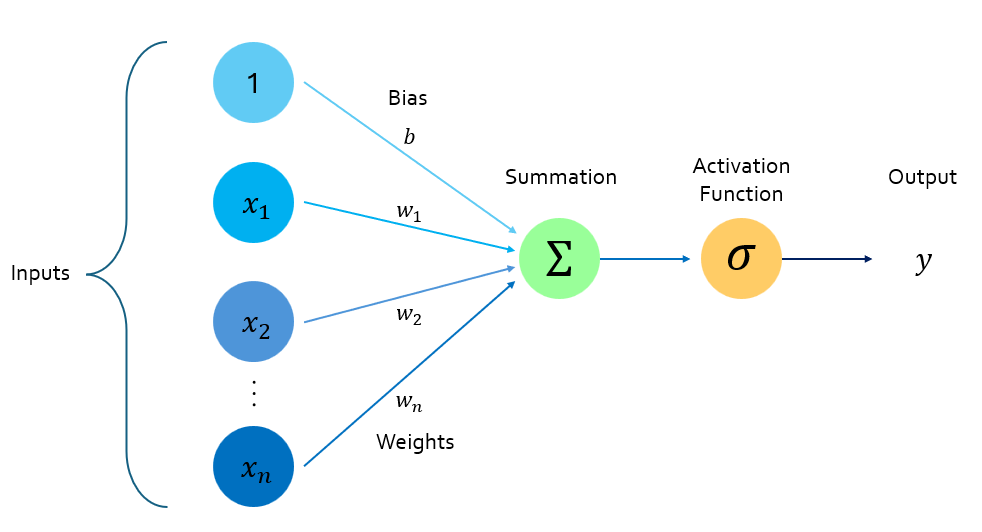
\includegraphics[width=12cm]{images/Theory-DL/ActFn.png}
    \caption{Perceptron}
    \label{fig:Perceptron}
  \end{figure}
\textbf{Activation functions} are usually non-linear functions to introduce non-linearity within the layers of neural networks, allowing them to learn and represent complex relationships in data. Common activation functions include sigmoid, tanh, ReLU (Rectified Linear Unit), and leaky ReLU. Activation functions transform the weighted sum of inputs $\mathbf{z}$ into the output signal $\mathbf{y}$, typically in the range between 0 and 1 (for sigmoid) or -1 and 1 (for tanh). Without the nonlinear transformation via the activation function, the network would be confined to solving merely linear problems. \\
% \begin{figure}[ht]
%     \centering
%     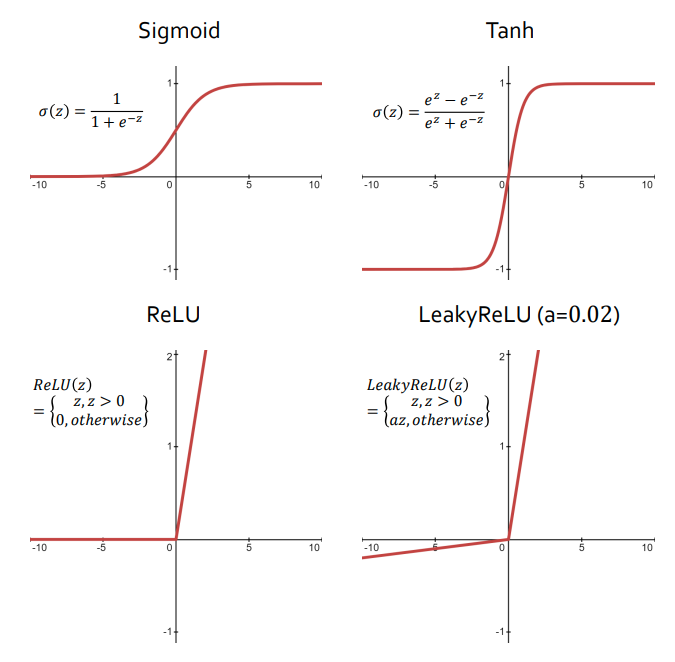
\includegraphics[width=8cm]{images/Theory-DL/ActGraphs.png}
%     \caption{Activation functions: (a) Sigmoid, (b) Tanh, (c) ReLU, and (d) Leaky ReLU}
%     \label{fig:ActGraphs}
%   \end{figure}
\textbf{Weights} in a neural network represent the strength of connections between neurons. They are learned parameters to adjust the influence of input signals on the neuron's output. \textbf{Biases} allow neural networks to model the offset from zero output, influencing the activation of neurons regardless of the input.\\
\textbf{Neural Networks (NNs)} consist of interconnected layers of perceptrons that process input data to produce output predictions. NNs can be represented as directed graphs, where nodes correspond to perceptrons, and edges depict connections between them. These connections typically carry weighted signals from one neuron's output to another neuron's input. Based on the structure of this connection graph, neural networks can be broadly classified into feed-forward neural networks and recurrent neural networks.\\
In \textbf{feed-forward neural networks}, information flows only in one direction, from the input layer through one or more hidden layers to the output layer. Each layer processes the input data independently, and the output of one layer serves as the input to the next layer. The connections between neurons do not form directed cycles, ensuring that the network architecture is acyclic. Multi Layer Perceptrons (MLPs) are the simplest feed-forward neural networks, and their architecture is described in Figure \ref{fig:MLP}. 
\begin{figure}[ht]
    \centering
    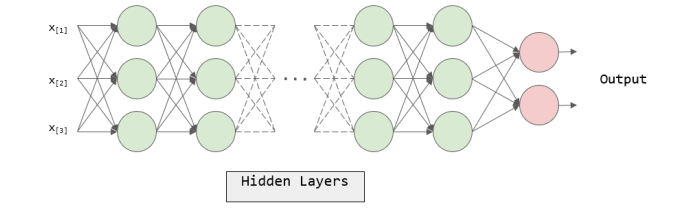
\includegraphics[width=10cm]{images/Theory-DL/MLP.png}
    \caption{Architecture of a Multi Layer Perceptron}
    \label{fig:MLP}
  \end{figure}
\textbf{Recurrent neural networks}, on the other hand, are designed to handle sequential data by allowing connections between neurons to form directed cycles. The feedback loops allow the network to maintain a memory of past inputs, making them suitable for tasks involving sequential data.
\section{Optimization}
Optimization involves adjusting the parameters of the neural network, such as weights and biases, to minimize a predefined objective function, typically referred to as the loss function. The optimization process iteratively updates the parameters based on the gradients of the loss function with respect to the network's parameters, aiming to converge to a set of optimal parameters that yield the best performance on the given task. Some important aspects of the optimization process are discussed in the following subsections. 
\subsection{Loss function}
The loss function quantifies the difference between the model's predictions and the actual target values. It represents the measure of how well the model is performing on the training data. Common loss functions include mean squared error (MSE) for regression tasks and categorical cross-entropy for classification tasks. The loss function $\mathcal{L}(\theta)$ is defined as: 
\begin{equation}
    \mathcal{L}(\theta)=\frac{1}{N} \sum_{i=1}^N L\left(y_i, \hat{y}_i ; \theta\right)
    \end{equation}
Here, $\theta$ represents the parameters of the neural network being optimized, such as weights and biases, $y_i$ is the ground truth and $\hat{y}_i $ is the model prediction. The loss function $\mathcal{L}(\theta)$ depends on these parameters, and it is computed as the average of the individual loss $L\left(y_i, \hat{y}_i ; \theta\right)$ over all training examples.
\subsection{Backpropagation}
Backpropagation is a fundamental algorithm used to compute the gradients of the loss function with respect to the parameters (weights and biases) of the neural network. It involves propagating the error backward from the output layer to the input layer, updating the parameters along the way to minimize the loss. The gradients are computed using the chain rule of calculus, enabling efficient optimization of the network's parameters. Mathematically, the gradients $\nabla_\theta \mathcal{L}(\theta)$ of the loss function are computed as,
\begin{equation}
    \nabla_\theta \mathcal{L}(\theta)=\frac{1}{N} \sum_{i=1}^N \nabla_\theta L\left(y_i, \hat{y}_i ; \theta\right)
    \end{equation}
\subsection{Learning rate}
The learning rate is a hyperparameter that controls the size of the parameter updates, that is, the step size in the direction of the gradients computed by backpropagation. A higher learning rate may lead to faster convergence but risks overshooting the optimal solution, while a lower learning rate may result in slower convergence but more stable training. The parameter update rule with learning rate $\eta$ is given by:
\begin{equation}
    \theta_{t+1}=\theta_t-\eta \nabla_\theta \mathcal{L}(\theta)
    \end{equation}
Here, $\theta_{t+1}$ and $\theta_t$ represent the parameters at time step $t$ and $t+1$ respectively. Learning rate decay is often used to gradually reduce the learning rate during training with the help of learning rate schedulers such as,
\begin{itemize}
\item \textbf{Step decay} reduces the learning rate by a factor (typically constant) after a fixed number of epochs or iterations.
\item \textbf{Exponential decay} reduces the learning rate exponentially over time.
\end{itemize}
% \begin{figure}[ht]
%   \centering
%   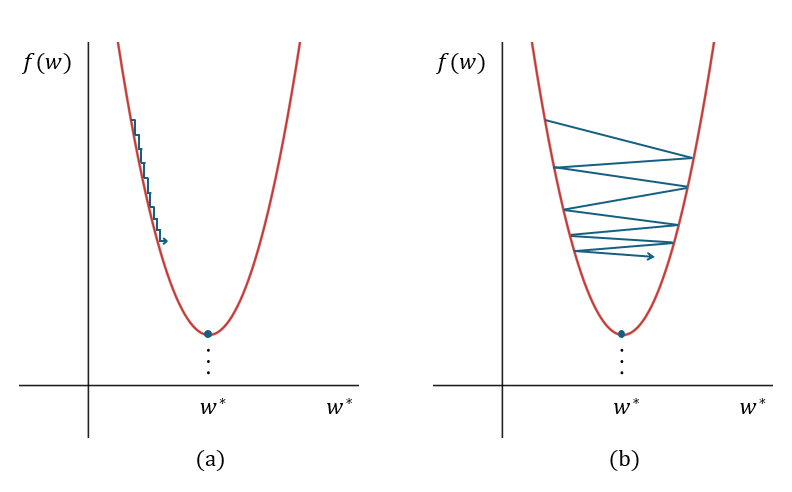
\includegraphics[width=10cm]{images/Theory-DL/LR.png}
%   \caption{Effect of Learning Rates}
%   \label{fig:LR}
%   \end{figure}
\subsection{Optimizer}
The optimizer is responsible for updating the parameters of the neural network based on the gradients computed during backpropagation. It determines the direction and magnitude of parameter updates to minimize the loss function efficiently. Popular optimizers include stochastic gradient descent (SGD), Adam, RMSProp, and AdaGrad.
\begin{enumerate}
\item \textbf{Stochastic Gradient Descent (SGD)} performs parameter updates using a fixed learning rate, which can lead to oscillations or slow convergence in the presence of sparse or noisy gradients.
\item \textbf{RMSProp (Root Mean Square Propagation)} adapts the learning rate for each parameter based on the magnitudes of recent gradients. It maintains a moving average of squared gradients for each parameter and divides the learning rate by the square root of this average to scale the parameter updates. RMSProp gets rid of the oscillations and slow convergence associated with fixed learning rates in SGD.
\item \textbf{AdaGrad (Adaptive Gradient)} algorithm adapts the learning rate for each parameter based on the history of gradients accumulated during training. It gives larger updates to parameters with smaller gradients, and vice versa. AdaGrad is useful for sparse data or problems with varying feature scales, as it automatically adjusts the learning rates for different parameters.
\item \textbf{Adam (Adaptive Moment Estimation)} maintains exponentially decaying moving averages of past gradients and past squared gradients for each parameter. Adam also incorporates bias correction terms to compensate for the initial bias towards zero at the beginning of training. The parameter update rule for Adam is given by
\begin{equation}
    \theta_{t+1}=\theta_t-\frac{\eta}{\sqrt{\hat{v}_t}+\epsilon} \cdot \hat{m}_t
    \end{equation}
where, $\hat{m}_t$ is the bias-corrected estimate of the first moment (mean) of the gradients, $\hat{v}_t$ is the bias-corrected estimate of the second moment (uncentered variance) of the gradients, and $\epsilon$ is a small constant to prevent division by zero.
\end{enumerate}
\section{Training of neural networks}
\subsection{Data partitioning}Data partitioning is a crucial step in deep learning in which the dataset is divided into separate subsets for training, validation, and testing. The data partitioned into training data is used to train the model, and validation data is used to tune hyperparameters and monitor performance. The testing data is used to evaluate the final model's generalization performance. The partitioning process ensures that the model's performance is assessed accurately on unseen data and provides independent datasets for training and evaluation. 
\subsection{Feature scaling}Feature scaling or normalization, is a preprocessing step aimed at bringing all input features to a similar scale. Features with large magnitudes can lead to large gradients during training, which may cause unstable behavior and make it challenging for the optimizer to find the optimum. Feature scaling mitigates this issue by reducing the range of feature values, thus preventing gradient instability and ensuring more reliable optimization. Common feature scaling techniques include,
\begin{enumerate}
\item Min-Max normalization: $x^{\prime}=\frac{x-x_{\min }}{x_{\max }-x_{\min }}$
\item Z-Score standardization: $x^{\prime}=\frac{x-\tilde{x}}{\sigma}$
\item Unit length scaling: $\mathrm{x}^{\prime}=\frac{\mathrm{x}}{\|\mathrm{x}\|}$
\end{enumerate}
\subsection{Weight initialization}
Weight initialization sets the initial values for the model's parameters before training begins. The loss landscape of deep neural networks is complex and non-convex, with multiple local minima. The initial weights dictate the local minimum the weights should converge to; thus, better initialization leads to improved model performance. There are different cases to consider for weight initialization: 
\begin{enumerate}
\item Initializing all weights to 0 or a constant leads to symmetrical gradients and weight updates across all neurons in the network during backpropagation. This results in the neurons learning identical features, causing the network to lose its representational capacity.
\item Large weights can lead to exploding gradients during training. Large weights can saturate activation functions, pushing them into regions of zero gradients (e.g., in sigmoid or tanh activations), hindering learning and resulting in slow convergence.
\item Small weights help prevent exploding gradients, as activations and gradients remain within a manageable range during training. However, extremely small weights results in small activations, leading to vanishing gradients. 
\end{enumerate}
% In summary, weight initialization is crucial for initializing neural networks effectively. 
Random initialization with small weights is a common practice in deep learning. Initializing weights to random values drawn from a suitable distribution with a zero mean and small variance breaks symmetry and helps prevent both vanishing and exploding gradients. It encourages each neuron to learn different features from the input data, promoting diverse representations and effective learning. Techniques like Xavier and Kaiming initialization further refine this process by adapting to the specific characteristics of activation functions.
\subsubsection{Xavier/Glorot initialization}
This technique initializes weights from a normal or uniform distribution with a zero mean. The variance of the distribution is adjusted based on the number of input neurons (fan-in) and output neurons (fan-out) as $\text{Var}(W) = \frac{2}{\text{fan}_{\text{in}} + \text{fan}_{\text{out}}}$. Xavier initialization is commonly used in shallow networks with symmetric activation functions, ensuring balanced weight initialization and stable training dynamics. 
\subsubsection{Kaiming/He initialization}
Kaiming initialization is designed for networks using non-linear activations like ReLU as seen in modern deep learning architectures. It initializes weights from a normal distribution with zero mean, adjusting the variance based on fan-in as $ \text{Var}(W) = \frac{2}{\text{fan}_{\text{in}}}$. Kaiming initialization helps mitigate the issue of vanishing gradients associated with ReLU activations, ensuring stable training and faster convergence.
\subsection{Regularization}
Regularization broadly refers to techniques used to prevent overfitting by imposing additional constraints on the model's parameters, i.e; by adding penalties to the loss function, thus discouraging complex models. Regularization penalizes large weights in the model, thereby promoting simpler models that generalize better to unseen data. Two common forms of regularization are L1 regularization (Lasso) and L2 regularization (Ridge). \\
L1 regularization encourages sparsity in the weights, performing feature selection by setting irrelevant weights to zero, making the model simpler and more interpretable. 
\[ \operatorname{Loss}_{\mathrm{L} 1}=\operatorname{Loss}_{\text {original }}+\lambda \sum_{i=1}^n\left|w_i\right| \]
L2 regularization encourages the weights to be spread out more evenly, preventing individual weights from becoming too large.
\[ \operatorname{Loss}_{\mathrm{L} 2}=\operatorname{Loss}_{\text {original }}+\lambda \sum_{i=1}^n w^2_i \]
Here, $\lambda$ is the regularization strength and determines the degree of penalty imposed on large weights. A smaller $\lambda$ value results in weaker regularization, allowing the model to fit the training data more closely but increasing the risk of overfitting. Conversely, a larger $\lambda$ value increases the regularization effect, resulting in a simpler model that generalizes better but may underfit the training data if set too high.
\subsubsection{Dropout}
Dropout is a regularization technique used in neural networks during training, where a random fraction of neurons is temporarily dropped out or ignored during forward and backward propagation. This prevents neurons from co-adapting and overfitting to the training data, promoting robustness and generalization. 
\subsection{Batch training and batch normalization}
Batch training is a technique in deep learning in which the model updates its parameters based on a subset (or batch) of the training data, rather than the entire dataset. The training data is divided into batches of fixed size, and the model computes the loss gradients for each batch using backpropagation. Since it computes the gradient updates based on an average over the samples in each batch, this reduces the variance in the gradient estimates compared to processing the entire dataset at once. This averaging effect stabilizes the gradients and prevents large fluctuations during training. \\
Selecting an appropriate batch size is crucial, as too small a batch size leads to frequent updates and noisy gradient updates. On the other hand, too large a batch requires more computational resources and memory despite providing precise gradient estimates, leading to stable optimization and faster convergence. Optimal batch size requires balancing the trade-off between computational efficiency and the quality of gradient estimates. \\                     
Another important term in this context is an epoch, which refers to a single pass through the entire training dataset. During one epoch, each batch is processed sequentially through the neural network. Once all batches have been processed, completing a full iteration over the entire dataset, one epoch is considered complete. Typically, training iterates over the entire dataset for multiple times or epochs until the model converges or a predefined stopping criterion is met. \\
% Batch normalization (BatchNorm) is another technique used in deep learning to stabilize and accelerate training by normalizing the activations of each layer within a mini-batch. 
Batch normalization (BatchNorm) is a technique to improve the stability and performance of neural networks by normalizing the activations of each layer. It operates on mini-batches of data and normalizes the input of each layer to have a mean of zero and a standard deviation of one. This is achieved by computing the mean and standard deviation of the activations across the batch, and then scaling and shifting the activations using learned parameters. The batch normalization transformation for a layer with input $x^{(1)}, x^{(2)}, \ldots, x^{(m)}$ is given as,
\begin{equation}
\begin{aligned}
& \mu_B=\frac{1}{m} \sum_{i=1}^m x^{(i)} \\
& \sigma_B^2=\frac{1}{m} \sum_{i=1}^m\left(x^{(i)}-\mu_B\right)^2 \\
& \hat{x}^{(i)}=\frac{x^{(i)}-\mu_B}{\sqrt{\sigma_B^2+\epsilon}} \\
& y^{(i)}=\gamma \hat{x}^{(i)}+\beta
\end{aligned}
\end{equation}
where $\mu_B$ and $\sigma_B^2$ are the mean and variance of the mini-batch $B$ of size $m$, $\epsilon$ is a small constant added to avoid division by zero, $\hat{x}^{(i)}$ is the normalized input, $\gamma$ and $\beta$ are learnable parameters (scale and shift), and $y^{(i)}$ is the output of the batch normalization layer.
\subsection{Overfitting and underfitting}
Overfitting and underfitting are two common phenomena that affect the performance and generalization ability of the model. Overfitting occurs when a model learns to perform well on the training data but fails to generalize to unseen data. The model becomes overly complex and specific to the training set, leading to poor generalization. Signs of overfitting include high training accuracy but low validation or test accuracy as the model memorizes training examples. Techniques such as regularization, dropout and early stopping can help prevent overfitting by reducing the model's capacity and complexity. \\
% This happens when the model captures noise or random fluctuations in the training data as if they were genuine patterns.
Underfitting occurs when a model is too simple to capture the underlying structure of the data. In this case, the model fails to learn the patterns present in the training data and performs poorly both on the training and unseen data. Underfitting often occurs when the model is too shallow or simple. Signs of underfitting include low training and validation accuracy. Increasing the model's capacity, adding more data, or improving feature engineering can help alleviate underfitting by allowing the model to capture more complex relationships in the data.
\subsection{Hyperparameters}\label{section:hyperparameters}
Hyperparameters in deep learning are fixed parameters set prior to the training process that are not learned from the data. They control various aspects of the learning process, such as the model architecture, optimization settings and the training procedure itself. Some important hyperparameters are the number of neurons per layer, number of layers, activation function, batch size, number of epochs, optimizer, loss function, weight initialization, dropout rate, and regularization strength. \\
Hyperparameter tuning is the process of selecting the optimal values for these hyperparameters to maximize the performance of the model on unseen data. It involves systematically searching through a predefined space of hyperparameters and evaluating the model's performance using a validation set or cross-validation. The goal is to find the hyperparameters that result in the best generalization performance, balancing between underfitting and overfitting.
\subsubsection{k-Fold cross-validation}
In k-fold cross-validation, the dataset is divided into $k$ subsets or folds, of approximately equal size. The model is trained $k$ times, each time using $k-1$ folds for training and the remaining fold for validation. This process is repeated $k$ times, with each fold used exactly once as the validation set. In the context of hyperparameter tuning, $k$-fold cross-validation helps evaluate the performance of different hyperparameter configurations. Instead of relying on a single validation set, this method averages the performance over multiple folds, providing a more stable estimate of the model's performance.
\section{Model evaluation metrics}
Model evaluation metrics are essential for assessing the performance of deep learning models. The loss function serves as a crucial metric for evaluating model performance, in addition to optimizing model parameters during training. In regression tasks, where the goal is to predict continuous values, common loss functions include the following:
\begin{itemize}
\item \textbf{Mean Absolute Error (MAE):} MAE measures the average absolute difference between the predicted values and the actual values:\[ \text{MAE} = \frac{1}{n} \sum_{i=1}^{n} |y_i - \hat{y}_i| \] Here, $y_i$ are the ground truth values, $\hat{y}_i$ are the predicted values, and $n$ is the number of samples. MAE is robust to outliers and does not penalize large errors heavily.
% \textbf{Mean Relative Error (MRE)}
\item \textbf{Mean Squared Error (MSE):} MSE measures the average squared difference between the predicted values and the actual values:\[ \text{MSE} = \frac{1}{n} \sum_{i=1}^{n} (y_i - \hat{y}_i)^2 \] MSE penalizes larger errors more heavily than MAE since errors are squared. This makes it more sensitive to outliers. 
\item \textbf{Root Mean Squared Error (RMSE):} RMSE is the square root of the average squared difference between the predicted values and the actual values: \[ \text{RMSE} = \sqrt{\frac{1}{n} \sum_{i=1}^{n} (y_i - \hat{y}_i)^2} \]RMSE is sensitive to outliers, similar to MSE, but is more interpretable as it is in the same units as the target variable.
\end{itemize}
\section{Convolutional Neural Networks (CNNs)}
CNNs are specialized neural networks designed to process grid-like data, such as images. They utilize convolutional layers and pooling operators to learn spatial hierarchies of features from input data, making them highly effective for tasks like image classification, object detection, and image segmentation.
\begin{figure}[ht]
    \centering
    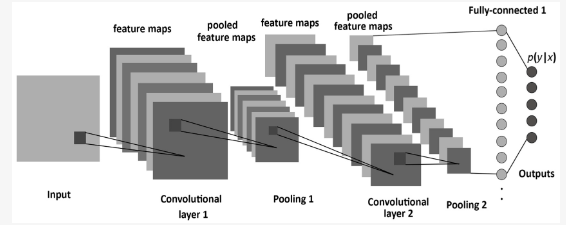
\includegraphics[width=10cm]{images/Theory-DL/CNN.png}
    \caption{Convolutional Neural Network}
    \label{fig:CNN}
  \end{figure}
\subsection{Convolutional layer}
The convolutional layer in a CNN consists of a set of learnable filters (kernels) that slide over the input data, performing element-wise multiplication and summing to produce feature maps. The convolution operation preserves the spatial relationship between pixels and learns local patterns like edges, textures, and shapes. Figure \ref{fig:Conv1} shows the working of a convolution kernel. 
\begin{figure}[ht]
    \centering
    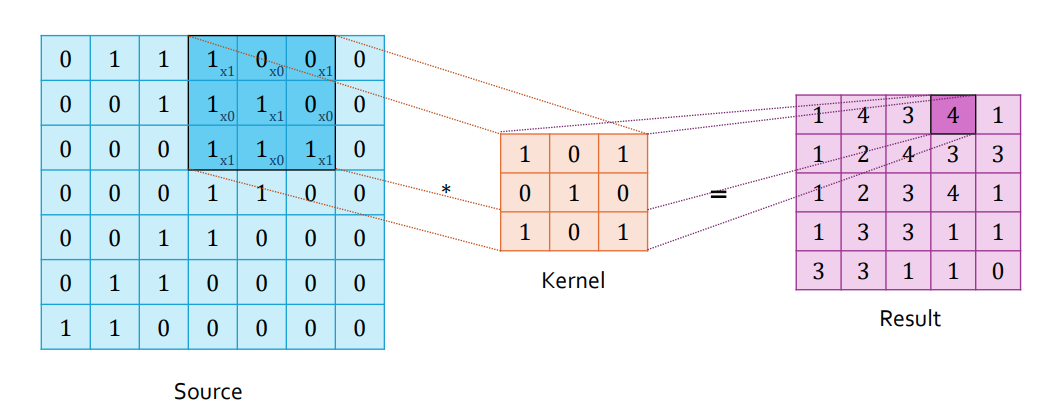
\includegraphics[width=14cm]{images/Theory-DL/Conv1.png}
    \caption{Convolutional Layer}
    \label{fig:Conv1}
  \end{figure}
\subsection{Pooling and unpooling} Pooling and unpooling operators perform effective downsampling and upsampling operations respectively, enabling hierarchical feature extraction while preserving spatial information. Pooling is a down-sampling operation commonly used in CNNs to reduce the spatial dimensions of feature maps. Max pooling and average pooling are popular pooling techniques that select the maximum or average value within each pooling region, respectively. These operations are depicted in Figure \ref{fig:Pool}. Conversely, unpooling layers, often used in upsampling, aim to reconstruct the original input resolution from the lower-dimensional representations generated by pooling. These layers typically store the indices of the maximum values during pooling and use them for upsampling. Nearest neighbor interpolation is a simpler upsampling method where each pixel in the input is replicated multiple times to form the output as can be seen in Figure \ref{fig:Unpool2}.
\begin{figure}[ht]
    \centering
    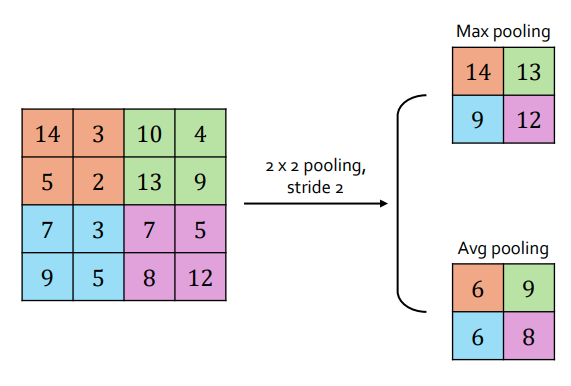
\includegraphics[width=8cm]{images/Theory-DL/Pool.png}
    \caption{Pooling}
    \label{fig:Pool}
\end{figure}
\begin{figure}[ht]
        \centering
        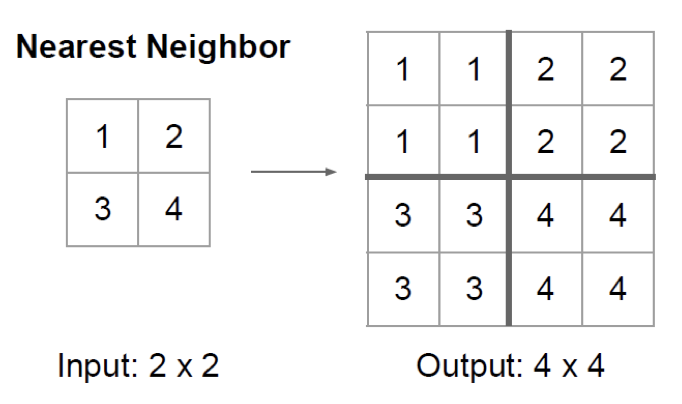
\includegraphics[width=8cm]{images/Theory-DL/NNUnpool.png}
        \caption{Unpooling}
        \label{fig:Unpool2}
    \end{figure}
\subsection{The U-Net architecture}
U-Net is a CNN consisting of a U-shaped network structure with a contracting path (encoder) followed by an expanding path (decoder), which enables precise segmentation of structures in medical images, such as cells, organs, or tumors. Some important components of the U-Net architecture are discussed below. 
\begin{figure}[ht]
    \centering
    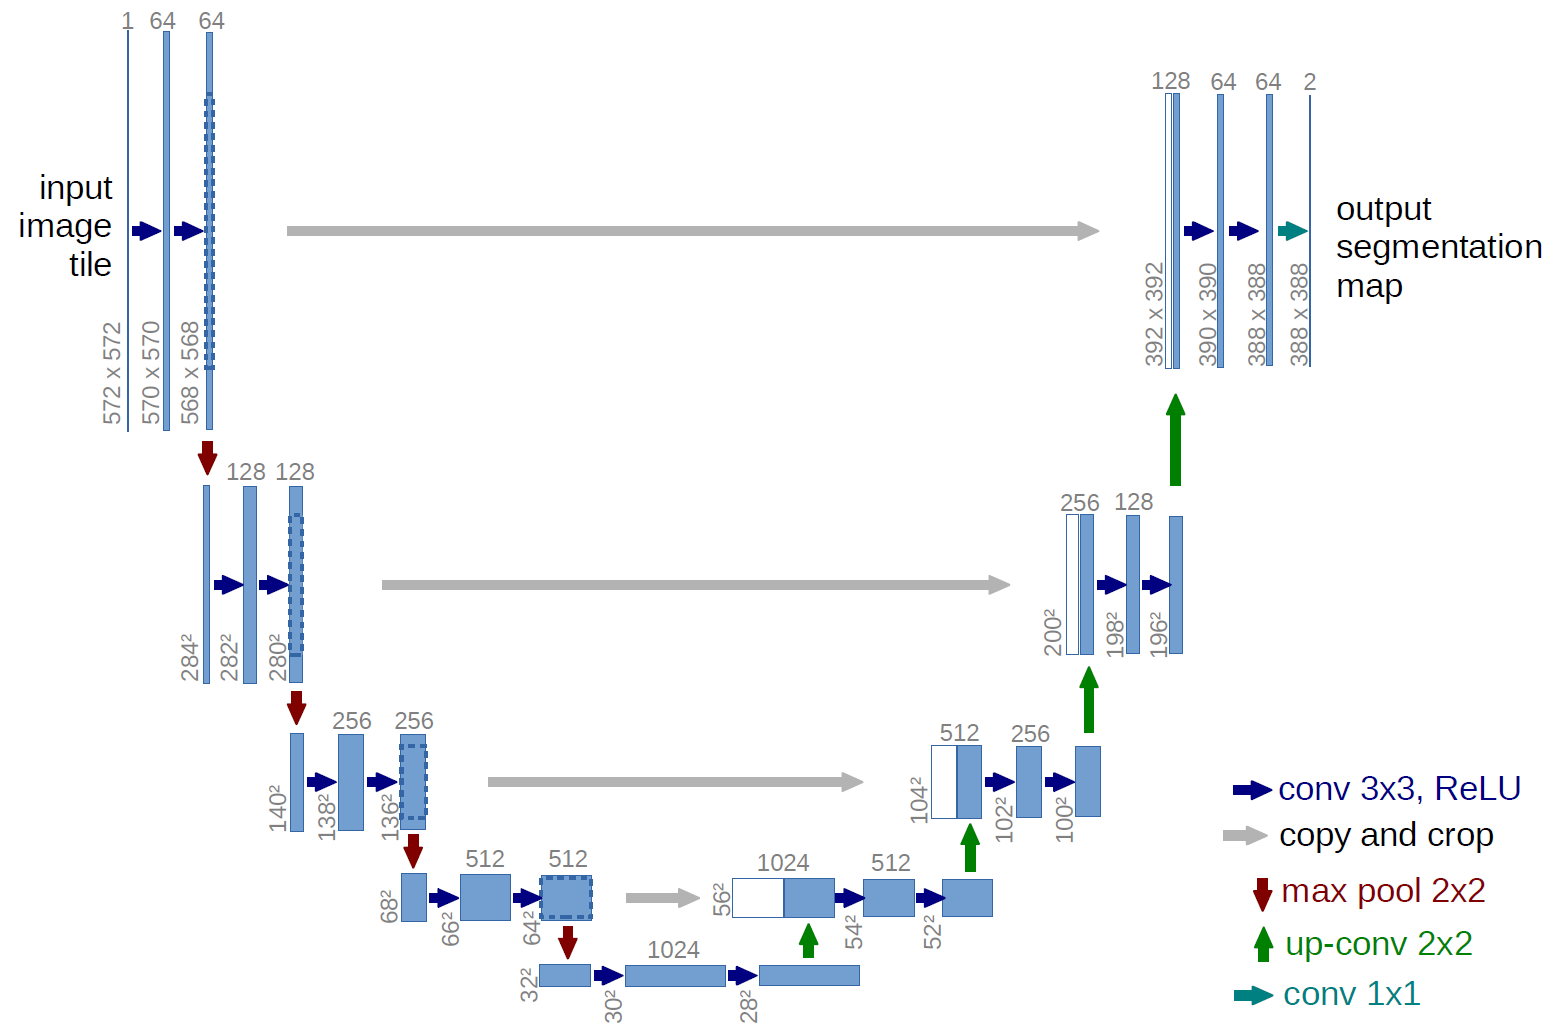
\includegraphics[width=12cm]{images/Theory-DL/UNet.png}
    \caption{U-Net Architecture}
    \label{fig:UNet}
\end{figure}
\begin{enumerate}
  \item The \textbf{encoder} comprises a series of down-convolutional and max pooling layers that gradually reduce the spatial dimensions of the input image while increasing the number of feature channels. This path extracts high-level features from the input image while preserving spatial context.
  \item The \textbf{decoder} consists of up-convolutional (transposed convolution) and concatenation layers that gradually increase the spatial dimensions of the feature maps while reducing the number of feature channels. This path generates segmentation masks by upsampling the low-resolution feature maps obtained from the encoder and combining them with high-resolution feature maps using skip connections.
  \item \textbf{Skip connections} or residual connections, are direct connections between layers at the same hierarchical level in the network. In the U-Net architecture, skip connections connect the encoder to the corresponding layers in the decoder. This enables the network to retain fine-grained spatial information from the encoder while recovering spatial details lost during downsampling. By directly linking the encoder and decoder layers, skip connections facilitate the flow of information across different scales, improving the model's ability to capture both local and global context.
\end{enumerate}
\begin{figure}[ht]
    \centering
    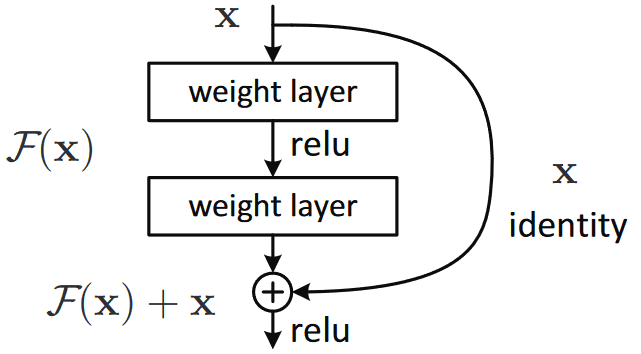
\includegraphics[width=6cm]{images/Theory-DL/Skip.png}
    \caption{Skip Connection}
    \label{fig:Skip}
\end{figure}
A notable observation pertinent to our current endeavor is the striking resemblance between the U-Net architecture and the V-cycle multi-grid method. Both employ a hierarchical structure wherein information is exchanged across varying resolutions.
\section{Graph Neural Networks (GNNs)}
A major limitation of CNNs is their inability to directly operate on irregular data formats, such as social networks, recommender systems, molecular structures, or citation networks. In 2017, Kipf and Welling \cite{kipf} introduced the Graph Convolutional Network (GCN), a foundational architecture that laid the groundwork for modern GNNs. Since then, numerous advancements and variants of GNNs have been proposed. In contrast to CNNs which are well-suited for grid-like structured data such as images, GNNs are tailored for data represented as graphs, which are characterized by non-Euclidean and irregular structures, where entities (nodes) and their relationships (edges) vary in connectivity and structure. GNNs excel in processing unstructured data by leveraging the inherent graph structure by dynamically aggregating information from neighboring nodes based on their connectivity. \\
Graphs are set up using nodes, edges, adjacency matrices, node attributes, and edge attributes. 
\begin{enumerate}
  \item \textbf{Nodes (\(V\))}: Nodes represent entities in a graph, such as users in a social network, atoms in a molecule, or words in a document. Formally, a graph can be denoted as \( G = (V, E) \), where \( V \) is the set of nodes.
  \item \textbf{Edges (\(E\))}: Edges define relationships or connections between nodes in a graph. Each edge \( e_{ij} \) connects node \( v_i \) to node \( v_j \), where \( v_i, v_j \in V \). The edge set \( E \) can be represented as a collection of tuples \( (v_i, v_j) \) indicating the connections between nodes.
  \item \textbf{Adjacency matrix (\(A\))}: An adjacency matrix is a binary $n \times n$ matrix representing the connections between nodes in a graph. For an undirected graph, \( A_{ij} \) is 1 if there exists an edge between nodes \( v_i \) and \( v_j \), and 0 otherwise. For directed graphs, the adjacency matrix may be asymmetric to represent the directionality of edges. The adjacency matrix \( A \) of a graph \( G = (V, E) \) can be defined as,
  \[
  A_{ij} = \begin{cases} 1 & \text{if } (v_i, v_j) \in E \\ 0 & \text{otherwise} \end{cases}
  \]
  \item \textbf{Node attributes and feature matrix(\(X\))}: Node attributes or features represent information associated with each node in the graph. These features can encode characteristics such as velocity, pressure, and temperature as node embeddings. The node feature matrix $X$ for a graph with \( N \) nodes and \( D \) features is a $N \times D$ matrix where each row corresponds to a node and each column represents a feature dimension, given by,
\begin{equation*}
  X = \begin{bmatrix} x_1^T \\ x_2^T \\ \vdots \\ x_N^T \end{bmatrix} \quad \text{ where,} \quad x_i = \begin{bmatrix} x_{i1} \\ x_{i2} \\ \vdots \\ x_{iD} \end{bmatrix}
\end{equation*}
where \( x_i \) represents the feature vector associated with node \(v_i \).
  \item \textbf{Edge weights or attributes (\(W\))}: Edge weights quantify the strength or intensity of relationships between nodes connected by edges. These weights can represent similarity measures, distances, or any other relevant information associated with edge connections. Similar to node weights, edge weights can be learned or predefined. 
\end{enumerate}  
\begin{figure}[ht]
  \centering
  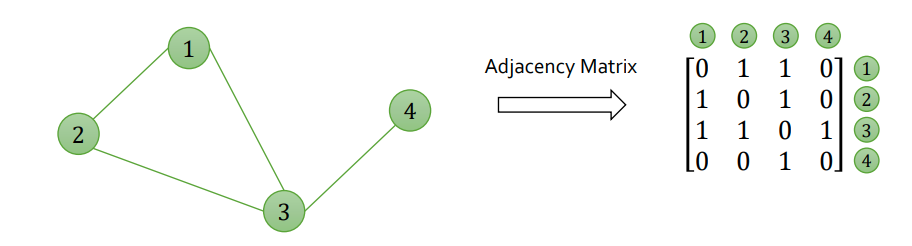
\includegraphics[width=12cm]{images/Theory-DL/AdjMat.png}
  \caption{Adjacency Matrix}
  \label{fig:AdjMat}
\end{figure}
GNNs leverage these components to perform message passing and aggregation operations across the graph structure, which are discussed below. \\
\subsection{Graph convolutions}
Graph convolutions update the feature representations of nodes in a graph by aggregating information from their neighboring nodes. There are two ways to perform graph convolution operations. In spectral convolution, graph signals are transformed into the spectral domain using techniques like graph Fourier transforms. Spatial convolution directly operates on the graph's topology and neighborhood structure, aggregating information from neighboring nodes without explicitly transforming the graph. Graph Convolutional Networks (GCNs), Graph Attention Networks (GATs), and GraphSAGE are common types of GNNs that utilize spatial convolutions. In this work, we only deal with spatial convolutions and refer to them as graph convolutions henceforth. The main steps involved in graph convolutions are as follows:
\begin{enumerate}
    \item \textbf{Message passing}: Nodes exchange messages with their neighbors, aggregating information from neighboring nodes. The message passed from node $v_j$ to node $v_i$ can be represented as:
        \[ m_{ij} = \frac{1}{c_{ij}} W h_j \]
        where $m_{ij}$ is the message from node $j$ to node $i$, $W$ is the learnable weight matrix, and $c_{ij}$ is a normalization factor.
    
    \item \textbf{Aggregation}:Nodes aggregate the messages received from their neighbors to update their own feature representations. The aggregated message $a_i$ for node $i$ can be computed as the sum or average of the incoming messages.
        \[ a_i = \sum_{j \in \mathcal{N}(i)} m_{ij} \]
    where $\mathcal{N}(i)$ denotes the set of neighboring nodes of $v_i$.
    \item \textbf{Update}: Nodes update their feature representations using the aggregated messages and their own features. The updated feature representation $h_i^{(l+1)}$ for node $i$ at layer $l+1$ can be computed as:
        \[ h_i^{(l+1)} = \sigma(a_i) \]
\end{enumerate}
These steps are performed iteratively across multiple layers of the GNN. At each layer, nodes update their feature representations based on the aggregated messages. The iterative propagation of messages allows nodes to incorporate information from distant parts of the graph and refine their representations over multiple layers. \\
Graph convolution operators typically exhibit local connectivity, where each node's representation is updated based on the information from its neighboring nodes.
This local connectivity property allows the model to capture localized patterns and dependencies within the graph structure. Weight sharing is a key aspect of graph convolutions, where the same set of learnable parameters (weights) is shared across different nodes in the graph. This allows for parameter efficiency and enables the model to generalize well to unseen nodes and graphs. 
% \subsection{Message passing}
% Message passing is a fundamental operation in GNNs where nodes exchange information with their neighbors in the graph. This mechanism enables nodes to aggregate and propagate information across the graph, allowing them to update their representations based on the local neighborhood structure. 
%%% \textbf{Message Computation:} Each node aggregates information from its neighboring nodes to compute a message. This aggregation process involves applying a function to combine features of neighboring nodes.\\
%%% \textbf{Message Aggregation:} After computing messages, each node aggregates the received messages to update its own representation. This aggregation operation typically involves summing or averaging the incoming messages. \\
% The message passing process can be represented as follows:
% \[
% m_{v \rightarrow u}^{(l)} = M^{(l)}(h_v^{(l)}, h_u^{(l-1)}, e_{vu})
% \]
% where,
% \begin{itemize}
%     \item $m_{v \rightarrow u}^{(l)}$ represents the message sent from node $v$ to node $u$ at layer $l$,
%     \item $M^{(l)}$ is a message function applied to the features of nodes $v$ and $u$ and the corresponding edge $e_{vu}$,
%     \item $h_v^{(l)}$ and $h_u^{(l-1)}$ are the feature vectors of nodes $v$ and $u$ at layers $l$ and $l-1$, respectively.
% \end{itemize}
% After computing messages, the aggregated message for node $u$ is obtained by combining messages from all neighboring nodes:
% \[
% m_u^{(l)} = \sum_{v \in \mathcal{N}(u)} m_{v \rightarrow u}^{(l)}
% \]
% where $\mathcal{N}(u)$ denotes the set of neighboring nodes of $u$.

\subsection{Graph pooling}
Graph pooling aggregates node representations across the entire graph to compute global graph-level features and create a coarser graph representation. It reduces the size of the graph representation while preserving important structural and relational information. By selecting representative nodes or aggregating node features, graph pooling enables GNNs to focus on relevant information while reducing computational complexity. Graph pooling also facilitates hierarchical feature learning by allowing GNNs to operate at multiple levels of granularity, enabling the model to capture both local and global patterns in the graph. The different types of graph pooling are:
\begin{enumerate}
\item \textbf{Top-k pooling} selects the top k nodes based on criteria such as node importance or feature values, and aggregates their information to create a coarser graph representation. This method retains the most informative nodes while reducing the size of the graph, making it suitable for tasks requiring node selection or summarization.
\item \textbf{Max pooling} selects the node with the maximum feature value from each neighborhood and aggregates their information to create a coarser representation of the graph. It emphasizes the most salient nodes in each neighborhood, capturing important features while reducing redundancy.
\item \textbf{Self-attention graph pooling} leverages attention mechanisms to dynamically weight the contributions of neighboring nodes based on their importance and similarity. It allows nodes to attend to relevant information in their neighborhoods, facilitating adaptive aggregation and effective summarization of the graph. This method is useful for capturing long-range dependencies and global patterns in the graph.
\end{enumerate}
% Graph pooling aggregates node features to produce a compact representation of the entire graph, which can be fed into subsequent layers or used for downstream tasks. \\
Graph unpooling is a complementary operation to graph pooling, aimed at upsampling or reconstructing the original graph representation after downsampling. While graph pooling creates a coarser representation, graph unpooling aims to recover the finer details and restore the original graph structure. Some common types of graph unpooling include,
\begin{enumerate}
\item \textbf{Max unpooling} is an unpooling strategy used in conjunction with max pooling. During max pooling, the locations of the maximum activations are stored. In max unpooling, these locations serve as masks to place the pooled values back into their original positions in the unpooled feature map.
\item \textbf{Nearest neighbor interpolation} aims to recover the original graph topology by identifying the nearest neighbors of pooled nodes in the coarse representation and reinstating unpooled nodes based on their proximity. It reconstructs edges between unpooled nodes and their nearest neighbors, restoring connectivity and preserving local structure.
%  Nearest neighbor unpooling is effective in capturing local relationships and structural patterns in the graph.
\end{enumerate}
% \subsection{Message Passing}
% \subsection{Graph Convolutions}
% \subsection{Graph Pooling and Unpooling}
\subsection{Hierarchical multi-resolution approach} 
\label{SO}
Multi-resolution approaches in the context of GNNs involve operating on graphs at multiple levels of granularity, similar to the multigrid method in numerical analysis. 
% In extending the multi-grid concept to the GNNs, a different approach is necessary compared to Convolutional Neural Networks (CNNs). 
Unlike CNNs, where downsampling operators automatically coarsen the mesh, in GNNs, we create a hierarchy of meshes with increasing complexity over the domain of interest. Hence, traditional pooling operators may not be suitable for GNNs, as they focus on selecting nodes to construct a coarse graph, which is unnecessary for mesh data. Instead, we can easily define operators that transform features from one mesh to the next, by generating a set of meshes with varying coarseness.\\
Creating a mesh hierarchy of different levels of coarseness can be performed by well-established techniques in numerical analysis. One commonly used algorithm for mesh construction is Delaunay triangulation, which maximizes the minimum angle of all triangles to avoid sliver triangles. This algorithm gradually inserts new nodes into the triangulation and connects them with their neighbors under specific rules. Incremental decimation is another mesh coarsening method that aims to reduce the number of points while preserving specific properties of the original mesh. It iteratively removes one vertex or edge with minimal changes until certain criteria are met. These techniques offer flexibility in creating mesh hierarchies, making them suitable for GNNs applied to mesh data.\\
\subsubsection{Sampling operator}
We introduce a sampling operator for converting data between two meshes, denoted as \(M_1\) and \(M_2\), inspired by the k-nearest interpolation proposed in PointNet++ \cite{pnpp}. Let \(z\) be a node from \(M_1\), and assume its \(k\) nearest neighbors on \(M_2\) are denoted as \(x_1, \ldots, x_k\). For a node feature \(f\), the interpolated feature \(f(z)\) is defined based on the features of \(x_i\) as,
\begin{equation}
  \mathbf{f}(\mathbf{z})=\frac{\sum_{i=1}^k w\left(x_i\right) \mathbf{f}\left(x_i\right)}{\sum_{i=1}^k w\left(x_i\right)} \text {, where } w\left(x_i\right)=\frac{1}{\left\|z-x_i\right\|_2}
  \end{equation}
With these operators, both upsampling and downsampling operators can be defined straightforwardly for developing multi-resolution architectures for mesh-based problems.
